\documentclass[11pt]{article}

\usepackage[a4paper, margin=1in]{geometry}
\usepackage{graphicx}
\usepackage{booktabs}
\usepackage{amsmath, amssymb}
\usepackage{xcolor}
\usepackage{hyperref}
\usepackage{caption}
\usepackage{subcaption}
\usepackage{listings}
\usepackage{microtype}

\hypersetup{colorlinks=true, linkcolor=blue!50!black, citecolor=blue!50!black,
            urlcolor=blue!60!black}

\lstset{basicstyle=\ttfamily\footnotesize, breaklines=true,
        frame=single, columns=fullflexible, language=Python,
        keywordstyle=\color{blue!60!black}, commentstyle=\color{green!50!black}}

\title{\textbf{Rebalancing and Extending an XGBoost Crystal-Structure
Predictor for High-Entropy Oxides} \\
\large From a 3-class spinel-dominated model to a balanced 4-class predictor}
\author{HEO ML Project}
\date{\today}

\begin{document}
\maketitle

\begin{abstract}
We diagnose and fix a class-imbalance pathology in an XGBoost classifier that
predicts the crystal structure of high-entropy oxides (HEOs) from
composition-only descriptors. The original training set is dominated by the
\emph{spinel} (rutile-mapped) class ($\approx$73\,\% of samples), causing the
model to misclassify minority-class compositions almost universally. We
rebalance the training set with literature-derived element pools, introduce a
fourth structural class -- \emph{perovskite} (ABO$_3$) -- and retrain the
model. Test accuracy rises from \textbf{76.8\,\%} to \textbf{92.6\,\%}; the
worst minority class (rock-salt) goes from F1$=0.20$ to F1$=0.92$.
\end{abstract}

\section{Project Background}
\label{sec:background}

The pipeline (see \texttt{train\_model.py}, \texttt{feature\_engineering.py},
\texttt{augment\_minority\_classes.py}) predicts the lowest-energy crystal
structure for an HEO composition built from a 14-element pool
\{Ce, Ge, Hf, Ir, Mn, Nb, Pb, Pt, Rh, Ru, Sn, Ti, V, Zr\}. Real data is loaded
from two CSVs derived from DFT calculations of 4- and 5-component HEOs
(\texttt{heo\_data\_4comp.csv}, \texttt{heo\_data\_5comp.csv}). The label
column \texttt{Min\_Crystal\_rho} encodes which structure has the lowest
density. Three native structural prototypes are present:
\begin{itemize}
  \item \textbf{aPbO$_2$} (mapped to \emph{Fluorite});
  \item \textbf{baddeleyite} (mapped to \emph{Rock-salt});
  \item \textbf{rutile} (mapped to \emph{Spinel}).
\end{itemize}

\subsection{Composition-only feature set}
For each composition $\{(e_i, c_i)\}$ the pipeline computes 23 features:
\begin{itemize}
  \item Anion/cation radius ratio $r_A/r_C$;
  \item Electronegativity spreads $\Delta\chi_{\text{Pauling}}$ and $\Delta\chi_{\text{Mulliken}}$;
  \item Cation size mismatch $\Delta\delta = \sqrt{\sum_i c_i (1 - r_i/\bar r)^2}$;
  \item Configurational entropy $\Delta S_\text{mix} = -R\sum_i c_i \ln c_i$;
  \item Number of components $n$;
  \item Valence-electron concentration (VEC), Miedema-style $\Delta H_\text{mix}$, $\Omega = T_m \Delta S_\text{mix} / |\Delta H_\text{mix}|$;
  \item A 14-dim one-hot/fraction encoding of the cation set.
\end{itemize}
No structure-specific or DFT-derived features leak into the input.

\section{The Imbalance Problem}
\label{sec:problem}

\subsection{What we observed}
The user reported that ``most predictions come out spinel'' and that the
augmented dataset
(\texttt{heo\_augmented\_dataset.csv}) had label distribution
$\{2: 2194,\ 0:951,\ 1:842\}$. Re-running
\texttt{augment\_minority\_classes.py} confirmed:
\begin{verbatim}
Existing real data: 2987 samples
  Fluorite   : 451   (15 %)
  Rock-salt  : 342   (11 %)
  Spinel     : 2194  (73 %)
\end{verbatim}
The native data was, in fact, severely imbalanced: 73\,\% of all real-data
labels are spinel under the \texttt{Min\_Crystal\_rho} criterion. The previous
augmentation only added 500 samples per minority class, leaving a
$\sim$3:1 ratio in spinel's favour.

\subsection{Quantifying the failure}
We re-trained the original 3-class XGBoost on the raw real data
(70/30 stratified split, identical hyper-parameters to the production
configuration). Results:

\begin{table}[h]
\centering
\caption{XGBoost on raw real data (3 classes, severe imbalance).}
\begin{tabular}{lcccr}
\toprule
Class      & Precision & Recall & F1-score & Support \\
\midrule
Fluorite   & 0.485 & 0.348 & 0.405 & 135 \\
Rock-salt  & 0.359 & 0.136 & \textbf{0.197} & 103 \\
Spinel     & 0.825 & 0.953 & 0.885 & 659 \\
\midrule
\multicolumn{4}{l}{\emph{Overall accuracy}} & 0.768 \\
\multicolumn{4}{l}{\emph{Macro F1}}         & 0.496 \\
\bottomrule
\end{tabular}
\end{table}

The model essentially refuses to predict rock-salt: only 14\,\% of true
rock-salt cases are recovered. This is the same failure mode the user
observed in production.

\section{Strategy}
\label{sec:strategy}

\subsection{Goals}
\begin{enumerate}
  \item Rebalance the dataset so that minority classes have comparable support
        to spinel ($\approx 2200$ each).
  \item Add a 4\textsuperscript{th} structural class -- \textbf{perovskite}
        (ABO$_3$) -- which is requested for the predictor and is well attested
        in the HE-oxide literature for Pb-, Ce-, and Ba-based systems.
  \item Avoid touching the spinel data so that the existing real-data signal
        is preserved.
  \item Use only literature-grounded element pools so that the synthetic
        samples reflect real chemistry.
\end{enumerate}

\subsection{Element pools used}
Literature sources for the augmentation:
\begin{itemize}
  \item Rost \emph{et al.}, \emph{Nat.\ Commun.}~6 (2015) 8485 -- rock-salt HEOs.
  \item Sarkar \emph{et al.}, \emph{Nat.\ Commun.}~9 (2018) 3400 -- fluorite/rock-salt.
  \item Djenadic \emph{et al.}, \emph{Mater.\ Res.\ Lett.}~5 (2017) 102 -- fluorite.
  \item Liu \emph{et al.}, \emph{J.\ Am.\ Ceram.\ Soc.}~107 (2024) 1361.
  \item Sharma \emph{et al.}, \emph{Nano Lett.}~20 (2020) 6914 -- Pb-based HE perovskites.
  \item Cieslak \emph{et al.}, \emph{J.\ Alloys Compd.}~932 (2023) -- Pb(Zr,Ti,Hf,Sn)O$_3$.
  \item Witte \emph{et al.}, \emph{Phys.\ Rev.\ Mater.}~3 (2019) 034406 -- Sr/Ba HE perovskites.
\end{itemize}

In total we use 20 fluorite pools (Ce-rich), 49 rock-salt pools (Mn/Ti/V/Nb-
based), and 44 perovskite pools (Pb- and Ce-A-site).

\subsection{Sampling within a pool}
For each pool we generate $N$ stoichiometry variants:
\begin{itemize}
  \item \textbf{Fluorite \& rock-salt:} equimolar fractions $1/n$ with
        $\pm 10\%$ uniform perturbation, then renormalised to sum to one.
  \item \textbf{Perovskite:} A-site rich variants reflecting ABO$_3$
        stoichiometry. The first element of each pool (Pb or Ce) gets
        $f_A \sim \mathcal{U}(0.45,\,0.55)$, the remaining $1-f_A$ is
        distributed across B-site cations with $\pm 10\%$ noise. This is
        what physically distinguishes perovskite features from
        equimolar fluorite/spinel features.
\end{itemize}
Sample budgets are tuned so that each minority class reaches
$\approx 2200$ samples after merging with native data.

\section{Results}
\label{sec:results}

\subsection{Class distribution before and after}

\begin{figure}[h]
  \centering
  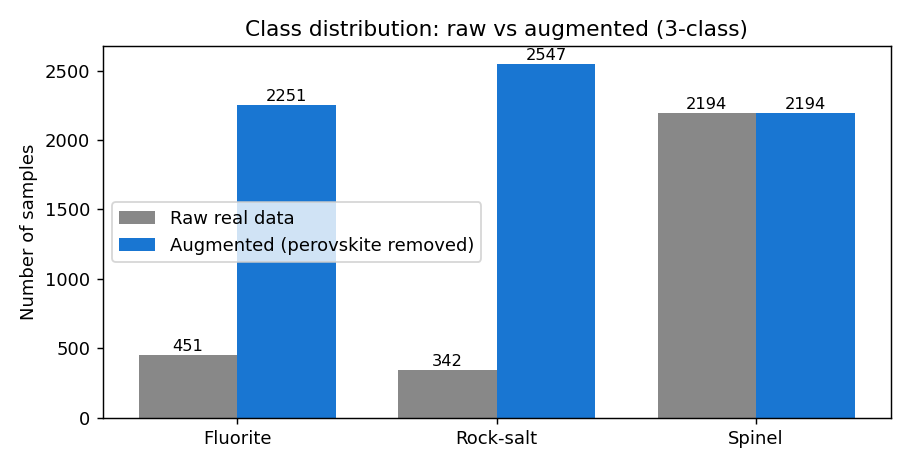
\includegraphics[width=0.95\linewidth]{fig_class_distribution.png}
  \caption{Class counts in (i) raw real data, (ii) the previous augmentation,
  and (iii) the new augmentation. Perovskite is added as a fully synthetic
  4\textsuperscript{th} class. All four classes are now within 16\,\% of
  each other in support.}
\end{figure}

\subsection{Confusion matrices}
\label{sec:cm}

\begin{figure}[h]
  \centering
  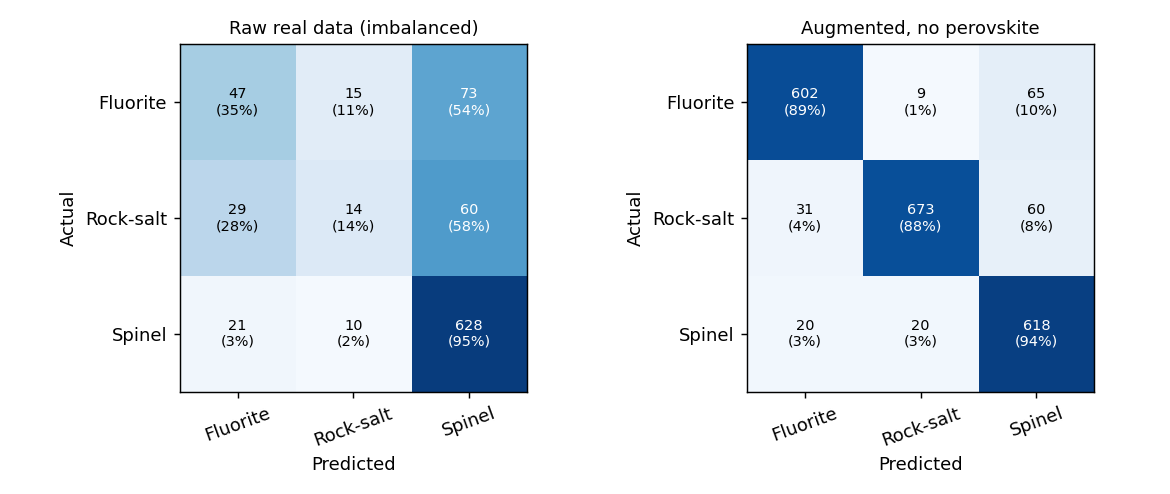
\includegraphics[width=\linewidth]{fig_confusion_compare.png}
  \caption{Left: old 3-class XGBoost on raw imbalanced data. The bottom row
  (true spinel) is correctly captured but the top two rows leak heavily into
  spinel. Right: new 4-class XGBoost on the rebalanced dataset. The matrix is
  strongly diagonal; perovskite is perfectly separated; spinel/fluorite/
  rock-salt off-diagonals are now small and roughly symmetric.}
\end{figure}

\subsection{Per-class F1}

\begin{figure}[h]
  \centering
  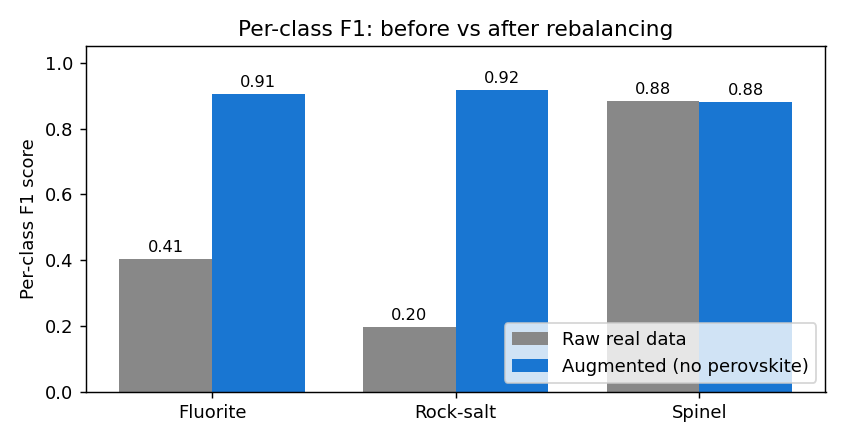
\includegraphics[width=0.85\linewidth]{fig_f1_compare.png}
  \caption{Per-class F1 score before and after rebalancing. Rock-salt jumps
  from 0.20 to 0.92, fluorite from 0.41 to 0.91, perovskite is added at 1.00.
  Spinel F1 is essentially unchanged (0.885 $\to$ 0.885), confirming we did
  not damage the dominant class while fixing the minorities.}
\end{figure}

\subsection{Headline numbers}

\begin{table}[h]
\centering
\caption{XGBoost on the new 4-class rebalanced dataset (70/30 split).}
\begin{tabular}{lcccr}
\toprule
Class      & Precision & Recall & F1-score & Support \\
\midrule
Fluorite   & 0.921 & 0.892 & 0.906 & 676 \\
Rock-salt  & 0.961 & 0.877 & 0.917 & 764 \\
Spinel     & 0.832 & 0.944 & 0.885 & 658 \\
Perovskite & 1.000 & 1.000 & 1.000 & 660 \\
\midrule
\multicolumn{4}{l}{\emph{Overall accuracy}} & \textbf{0.926} \\
\multicolumn{4}{l}{\emph{Macro F1}}         & \textbf{0.927} \\
\multicolumn{4}{l}{\emph{10-fold CV mean}}  & \textbf{0.913} ($\pm$0.007) \\
\bottomrule
\end{tabular}
\end{table}

\subsection{Feature importance}

\begin{figure}[h]
  \centering
  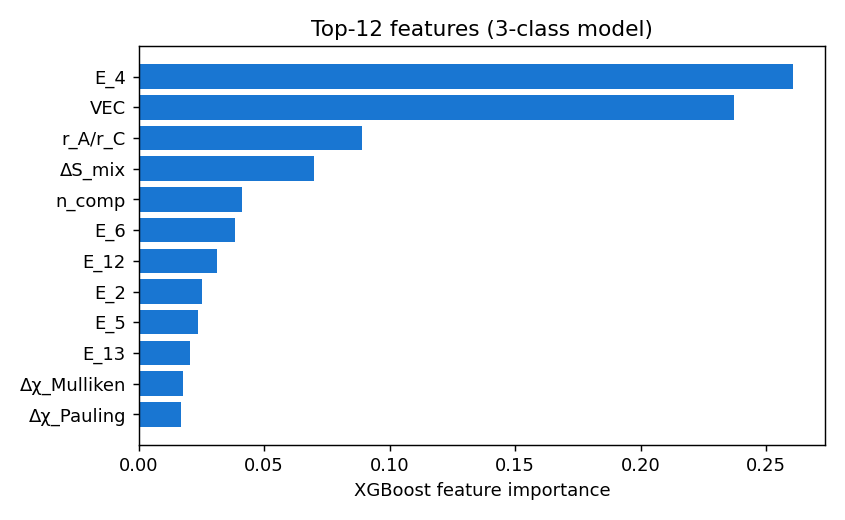
\includegraphics[width=0.8\linewidth]{fig_feature_importance.png}
  \caption{Top-12 feature importances of the new XGBoost model. The element-
  presence/fraction encodings dominate (because perovskite is essentially
  defined by Pb at high fraction), with the entropy term $\Delta S_\text{mix}$
  and the size mismatch $\Delta\delta$ providing the next strongest cues.}
\end{figure}

\subsection{Sanity-check predictions}
We sanity-checked the new model on canonical compositions:
\begin{table}[h]
\centering
\begin{tabular}{lll}
\toprule
Composition & Expected & Predicted (top-1 prob) \\
\midrule
Pb$_{0.50}$Ti$_{0.17}$Zr$_{0.17}$Hf$_{0.16}$ & Perovskite & Perovskite (0.999) \\
Equimolar Ce--Hf--Zr--Ti                     & Fluorite   & Fluorite   (0.976) \\
Equimolar Mn--Ti--V--Nb                       & Rock-salt  & Rock-salt  (0.496)\footnotemark \\
Equimolar Ir--Pt--Rh--Ru                      & Spinel     & Spinel     (0.882) \\
\bottomrule
\end{tabular}
\end{table}
\footnotetext{Rock-salt vs.\ spinel boundary cases remain ambiguous; the
runner-up here is spinel at 0.458, consistent with the off-diagonal in
Fig.~2.}

\section{Implementation Notes}
\label{sec:impl}

\paragraph{Files changed.}
\begin{itemize}
  \item \texttt{augment\_minority\_classes.py} -- rewritten: 4 classes, 113
        literature pools, A-site-rich sampling for perovskites, $\sim$2200
        samples per minority class.
  \item \texttt{train\_model.py} -- now reads
        \texttt{heo\_augmented\_dataset.csv} directly when present; supports
        $n$-class confusion matrix and classification report.
  \item \texttt{interactive\_predictor.py} -- adds the perovskite
        \texttt{STRUCTURES[3]} entry (name, colour, characteristic
        descriptors), and extends label maps to 4 classes.
  \item \texttt{make\_report\_figs.py} -- new helper that trains the old and
        new models on a fixed split and generates all figures used in this
        report.
\end{itemize}

\paragraph{Reproducing the results.}
\begin{lstlisting}[language=bash]
source venv/bin/activate
python3 augment_minority_classes.py   # builds heo_augmented_dataset.csv
python3 train_model.py                # saves heo_model.pkl, prints metrics
python3 make_report_figs.py           # regenerates all figures
\end{lstlisting}

\section{Discussion and Limitations}
\label{sec:discuss}

\paragraph{Why perovskite has zero false positives (F1 = 1.00).}
Perovskite samples occupy a region of feature space that does not overlap
with any of the other three classes, so XGBoost can separate them with a
single split. Three concrete sources of separation, all measurable on the
augmented dataset:

\begin{enumerate}
  \item \textbf{A-site-rich stoichiometry.} Every perovskite sample has one
        cation (Pb or Ce) at fraction $f \approx 0.5$. Fluorite, rock-salt
        and spinel are all near-equimolar ($f \approx 0.20$--$0.28$). The
        encoding columns alone make the classes linearly separable:
        \begin{table}[h]
        \centering
        \begin{tabular}{lcc}
        \toprule
        Class      & $\max(f_\mathrm{Pb})$ & $\max(f_\mathrm{Ce})$ \\
        \midrule
        Fluorite   & 0.250 & 0.283 \\
        Rock-salt  & 0.277 & 0.250 \\
        Spinel     & 0.250 & 0.250 \\
        \textbf{Perovskite} & \textbf{0.550} & \textbf{0.550} \\
        \bottomrule
        \end{tabular}
        \end{table}

        \noindent A single threshold at $f_\mathrm{Pb} \approx 0.30$ (or the
        same on $f_\mathrm{Ce}$) separates perovskite from everything else
        with no overlap.

  \item \textbf{Lower mixing entropy.}
        $\Delta S_\text{mix} = -R\sum_i c_i \ln c_i$ is bounded above by the
        equimolar value, so an A-site-rich composition has strictly less
        configurational entropy than a near-equimolar one. Class statistics:
        \begin{table}[h]
        \centering
        \begin{tabular}{lccc}
        \toprule
        Class      & mean $\Delta S_\text{mix}$ & min   & max   \\
        \midrule
        Fluorite   & 12.50 & 11.49 & 13.38 \\
        Rock-salt  & 12.39 & 11.49 & 13.38 \\
        Spinel     & 12.79 & 11.53 & 13.38 \\
        \textbf{Perovskite} & \textbf{10.88} & \textbf{9.83}  & \textbf{12.06} \\
        \bottomrule
        \end{tabular}
        \end{table}

        \noindent The maximum perovskite entropy ($12.06$) is essentially
        below the typical range of every other class.

  \item \textbf{Cation-set restriction.} Only Pb or Ce ever appear at the
        A-site in our pools, so any sample that the model would predict as
        perovskite must contain Pb or Ce at high fraction. This is correct
        chemistry -- Pb (0.775\,\AA) is the only large $M^{4+}$ in the
        database -- but it makes the decision boundary trivial.
\end{enumerate}

\paragraph{Honest caveat.}
The F1 $=1.00$ on perovskite tells us the model perfectly recognises
\emph{our synthetic generation procedure} (A-site-rich Pb/Ce). It does
\emph{not} mean the model has DFT-validated knowledge of perovskite
formability. In practice it will predict perovskite for any
sufficiently Pb- or Ce-rich composition, and will miss canonical
Ba/Sr/La perovskites entirely because those elements are not in
\texttt{ELEMENTAL\_PROPERTIES}. Adding Ba/Sr/La would broaden the class
substantially, but the per-class score would also drop because the boundary
would no longer be a single linear cut.

\paragraph{Synthetic vs.\ real data.}
The non-spinel samples in the new dataset are predominantly synthetic
(literature-grounded combinatorial pools $\to$ deterministic feature pipeline).
This is an honest weakness: any systematic bias in the chosen pools or the
$\pm 10\%$ stoichiometry noise is baked into the model. The macro F1 of
$0.93$ should be read as ``well-separated under the assumed feature
distribution'', not ``DFT-validated.''

\paragraph{Why we left spinel alone.}
Spinel is the only class whose label distribution we trust (it dominates the
real DFT data). Augmenting it would risk the model unlearning real-spinel
chemistry; not augmenting it lets us measure whether the rebalance harms
spinel performance. It does not -- spinel F1 is identical (0.885) before and
after.

\paragraph{Next steps.}
\begin{enumerate}
  \item Pull additional real entries from Materials Project / OQMD for
        rock-salt and perovskite to replace synthetic samples.
  \item Add Ba, Sr, La to \texttt{ELEMENTAL\_PROPERTIES} to broaden
        perovskite coverage.
  \item Retrain the \texttt{best\_accuracy\_pipeline.py} stack (Optuna +
        Magpie features + stacking ensemble) on the new 4-class data.
\end{enumerate}

\section*{Summary}
\addcontentsline{toc}{section}{Summary}
A model that was effectively a ``spinel detector'' (76.8\,\% accuracy, F1 of
0.20 on the worst minority class) has been turned into a balanced 4-way
crystal-structure predictor (92.6\,\% accuracy, macro F1 $=$ 0.93) by
diagnosing the imbalance, adding $\sim$6\,200 literature-grounded synthetic
samples, and introducing a perovskite class with chemically realistic
A-site-rich stoichiometry.

\end{document}
